\documentclass[conference]{IEEEtran}

\usepackage{amssymb,amsmath}
\usepackage{wrapfig}
\usepackage{multirow}
\usepackage{graphicx}
\usepackage{algorithm}
\usepackage{algorithmic}
\usepackage{times}
\usepackage{cite}
\usepackage{url}
\usepackage{booktabs}
\usepackage{subfigure}
\usepackage{fancybox}
\usepackage{color}
\usepackage{array}
\usepackage{subfigure}
\usepackage{balance}
\usepackage{epstopdf}
\usepackage{array}


\newcommand{\everton}[1]{\textcolor{blue}{{\it [Everton: #1]}}}
\newcommand{\todo}[1]{\colorbox{yellow}{\textbf{[#1]}}}


\newcommand{\conclusionbox}[1]{%
	\vspace{2mm}
	\framebox[0.45\textwidth][c]{%
		\parbox[b]{0.42\textwidth}{%
			{\it #1}
		}
	}
	\vspace{2mm}
}

\newcommand{\rqi}{\textbf{}}
\newcommand{\rqii}{\textbf{}}
\newcommand{\rqiii}{\textbf{}}

\begin{document}
\title{Paper Title here}

\author{\IEEEauthorblockN{Everton da S. Maldonado}

\IEEEauthorblockA{Department of Computer Science and Software Engineering\\Concordia University,
Montreal, Canada\\
\url{everton.maldonado@gmail.com}}}

\maketitle

\begin{abstract}
\end{abstract}

\IEEEpeerreviewmaketitle

\section{Introduction}
\label{sec:introduction}
Software system becomes more important each passing day and the effort to produce good and successful software projects increases at the same pace. In an ideal world a project  should be delivered on time, inside the budget and with high quality. We know by experience that is very  difficult to balance these elements, and they are mostly likely to be indirectly proportional. Quality is very important though, and many approaches have been proposed to ensure software quality. However there is always a tradeoff between quality and and resources. For example, developers often take shortcuts to meet release deadlines, fix last minute bugs, etc.

A new area that studies this phenomena is Technical Debt. The term technical debt is used to express faults and non-optimal solutions that are taken conscientiously in a software project in order to achieve short term goals. Usually  this decisions allows the project to move faster towards its goal but there will be an increased cost to maintain this software in the long run. Prior work \cite{Lim2012Software} showed that technical debt is unavoidable and that there is different types of technical debt, like design debt, test debt, documentation debt, defect debt, etc.  

The technical debt metaphor is widely used in industry and the research in this area is expanding as well. However, in topics like defect debt, different works has a divergent opinion. Some studies says that defect technical debt does not exists \cite{Kruchten2013GSOFT} as in the other hand, there are studies supporting the existence of defect technical debt \cite{Seaman201125}. We argue that there are different kinds of defects in a project, and that some of them can be characterized as defect technical debt, although not all of defects are necessarily  a defect technical debt. 

Our goal is to understand, characterize and model Defect Debt, being able to distinguish Defect Debt from other Bugs.

In this paper, we extract more than 139,000 commits and analyze more than 67,000 bug reports from one large open source software. We performe a empiracal study on Google Chrome to answer our research questions. 

Fisrt, we analyze 25 releases from Chrome grouping the number of reported bugs and fixed bugs for each one of them. Based on the result of this analysis we found a pattern that can categorize Defect Debt and Bugs. We found that Bugs are more urgent defects, that are fixed in the same release as reported or in the immediatly next one. However, Defect debt lingers in the system for a long time, but eventually get fixed. In the analyzed project the avarage percentage of Bugs are of 69.55\% and Defect Debt is of 30.44\%.

Second, we analyze the total number of open bugs in the system and the number of Defect Debt. Then we classify the commits accordingly with their intention. We use this information in to undertand how Defect Debt impacts the addition of new features. Based on our result we find that there is no direct negative relation between the number of Defect Debt and the addition of new features. 

Third, we collect several metrics and propose a model to Defect Debt, we find that it is possible to build such a model, but it is necessary to treat the data in a more granular level (i.e., file level). 

The rest of the paper is organized as follows: Section~\ref{sec:related_work} presents the related work, followed by Section~\ref{sec:approach} that details our approach. We present our case study results in Section~\ref{sec:results}. The threats to validity of our work are discussed in Section~\ref{sec:threats_to_validity}. Section~\ref{sec:conclusion} lists the ours conclusions and future work. 

\section{Related Work}
\label{sec:related_work}
Our work differs from previous work because a Defect Debt is a know issue to the development team whereas a Dormant Bug is a defect that is hidden for a long period of time and eventually it crash. In other words Defect Debt is know option not an accident.

\section{Approach}
\label{sec:approach}
\begin{figure*}[thb!]
  \caption{Approach overview}
  \centering
  \label{fig:approach}
  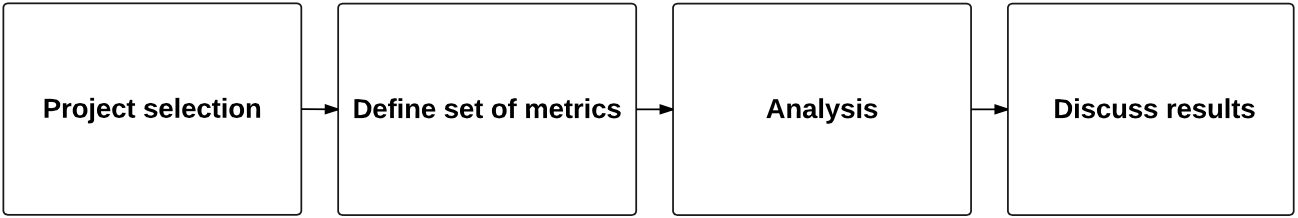
\includegraphics[width=1\textwidth]{figures/approach}
\end{figure*}

The goal of our project is to distinguish Defect Debt from Bugs. In order to do that we conducted a study using one large open source project, Google Chrome. We present our approach overview in \ref{fig:approach}. First, we extract data from the source code and from the issuer tracker repositories. Second,  we process the data to find relevant attributes and link them together. Third, we define our set of metrics and models. Then we analyze our results and answer the research questions. In the following sections we explain in details each one of the steps in our approach.   

\subsection{Data Extraction}

We use Google Chrome to conduct our study. Chrome is a large, mature open source software mostly written in C/C++. The criteria to select this project are its size, the easy access to its source code repository and to the its issuer tracker. Other than that, we had at our disposal some of the desired data that was used in a previous study. This data contained 47.938 html files and 5 tables. Each one of the files represent a bug extracted from the issue tracker. The tables contains the necessary information to link issues files, bugs and commits together. 

To complement the data necessary to our study, we extract from the Chrome Releases website \ref{chrome_releases} the release date of each stable version release, the tag of the release and the release number. Then we store this data in our database.
 
In order to have all the source code available we clone Chromium Git repository. 

\subsection{}


the issues files the the bug reported date and the number of comments that 

\section{Threats to validity}
\label{sec:threats_to_validity}
\noindent \textbf{External validity} consider the generalization of our findings. All of our findings were derived from one open source project. To minimize external validity, we chose a large open source project. That said, our results may not generalize to other open source or commercial projects.

\section{Conclusion and Future work}
\label{sec:conclusion}
In our study we analyzed Google Chrome a large open source project to understand the different characteristics between Bugs and Defect Debt. 

We show in our approach how to extract, process and link data from this project. We also explain the different metrics that we selected and how we group the metrics into releases. 

We find that it is possible to characterize Defect Debt from bugs. Bugs are more impacting defects, and get fixed in the reported or in the next release. Whereas Defect Debt may linger in the system for a long time, but eventually it get fixed. We draw this conclusion after analyzing the behavior of the fixes throughout 25 different releases of the project. Based on the results, the average percentage of Bugs is of 69.55\%, and Defect Debt is of 30.44\%.

We found that the defect debt does not impact negatively the addition of new features. Is important to notice that we are not considering other aspects that may impact quality.  

Although the correlations between the measures are not high their directions gives us insights to add more meaningful metrics.

One possible way to improve the Defect Debt model is to calculate the effective size for the regression. Other possibility is to reformulate the problem. Changing the granularity of the analysis to the level file instead of the release level. 

In a future work we plan to include in our analyze the severity of the issues. In our current analysis we do not take this factor in consideration. This will lead us further in the understanding of Defect Debt characterization, and prevent us of relying just on the assumption that only what is import get fixed. As a matter of fact, more research in this subject can provide empirical evidence for proving or rejecting this assumption.

\bibliographystyle{IEEEtran}
\bibliography{bib}

\end{document}
